\tikzset{arbre3/.style = {every node/.style = {minimum size = #1, circle, draw},
                          level distance =10mm, 
                          level 1/.style={sibling distance=48mm},
                          level 2/.style={sibling distance=24mm},
                          level 3/.style={sibling distance=12mm},
                         },
         arbre3/.default=8mm
        }
%----------------------------------------------------------------
%----------------------------------------------------------------
%----------------------------------------------------------------
\chapter{Tas} 
%----------------------------------------------------------------
%----------------------------------------------------------------
\vskip -2cm
%----------------------------------------------------------------
\section{Files de priorité}
%----------------------------------------------------------------
%----------------------------------------------------------------
\subsection{Type abstrait}
%----------------------------------------------------------------
Dans ce chapitre nous allons définir et implémenter un type de données efficace pour traduire le type abstrait de  file de priorité.
On rappelle qu'il s'agit de maintenir un ensemble d'objets d'un type fixé accompagnés d'une priorité qu'on suppose entière.

On veut pouvoir ajouter un élément en donnant sa priorité et exhiber ou retirer l'élément de priorité maximale.
On souhaite ainsi définir un type de donnée \type{'a fdp} de file de priorité dont les objets sont de type \type{'a} ainsi que les fonctions
%----------------------------------------------------------------
\begin{ocaml}
fpVide : 'a -> 'a fdp 
estVide : 'a fdp -> bool 
ajouter : 'a  -> int -> 'a fdp -> unit
premier : 'a fdp -> 'a 
enlever : 'a fdp -> unit
\end{ocaml}
%----------------------------------------------------------------
\begin{itemize}
\item \type{fpVide} demande un élément de type \type{'a} qui sera l'élément par défaut lorsque l'on aura besoin de tableaux.

\item \type{ajouter} modifie une file de priorité en lui ajoutant un coupe (élément, prioruté),

\item \type{premier} renvoie l'élément de priorité maximale dans une file de priorité sans la modifier.

\item \type{enlever} retire l'élément de priorité maximale d'une file de priorité.
\end{itemize}
%----------------------------------------------------------------
On remarque qu'on choisit une structure mutable.

\medskip

On peut parfois souhaiter pouvoir modifier la priorité d'un élément :
%----------------------------------------------------------------
\begin{ocaml}
changerPrio : 'a  -> int -> 'a fdp -> unit
\end{ocaml}
%----------------------------------------------------------------
On choisira ici de considérer cette fonction comme une généralisation de \type{ajouter} : si l'élément n'était pas dans la file de priorité, on l'ajoute.
Pour cela, il peut être utile d'introduire une fonction
%----------------------------------------------------------------
\begin{ocaml}
supprimer : 'a  -> 'a fdp -> unit
\end{ocaml}
%----------------------------------------------------------------
qui retire un élément de la file de priorité en fonction de sa valeur (et non de sa priorité).

La fonction de changement de priorité sera alors simple :
%----------------------------------------------------------------
\begin{ocaml}
let changerPrio x p fp =
   supprimer x fp;
   ajouter x p fp;;
\end{ocaml}
%----------------------------------------------------------------

\medskip

Bien entendu on souhaite une structure qui permette des fonctions dont les temps de calculs seront les plus petits possibles et dont l'occupation en mémoire est faible aussi.
%----------------------------------------------------------------
\newpage
%----------------------------------------------------------------
\subsection{Rappels : implémentations linéaires}
%----------------------------------------------------------------
%----------------------------------------------------------------
Il y a quatre possibilités pour l'implémentation avec les structures de données classiques
%----------------------------------------------------------------
\begin{itemize}
\item on peut choisir des listes ou des tableaux

\item pour chaque structure on peut soit trier lors de l'adjonction, soit extraire le maximum lors du calcul ou du retrait de l'élément de priorité maximale.
\end{itemize}
%----------------------------------------------------------------
%----------------------------------------------------------------
\begin{exo}{Listes triées}{}
Écrire les 7 fonctions définies ci-dessus au cas où le type concret est une liste maintenue triée :
\begin{ocaml}
type 'a fdp = {mutable contenu : ('a * int) list};;
\end{ocaml}
Quelles sont les complexités des fonctions ?
%----------------------------------------------------------------
\reponse
%----------------------------------------------------------------
\begin{ocaml}
let fpVide x = 
   {contenu = []};;

let estVide fp =
   fp.contenu = [];;
\end{ocaml}
  
\begin{ocaml}
let ajouter x p fp = 
   let rec inserer liste =
      match liste with
      |[] -> [(x, p)]
      |(y, k):: reste when p > k -> (x, p)::liste
      |t::q -> t::(inserer q) in
   fp.contenu <- inserer fp.contenu;;
\end{ocaml}

\begin{ocaml}
let premier fp =
   fst (List.hd fp.contenu);;
   
let enlever fp =
   fp.contenu <- List.tl fp.contenu;;
\end{ocaml}

Si un élément à supprimer n'existe pas, on laisse la file inchangée.
\begin{ocaml}
let rec supprimer x fp =
   let rec oter liste =
      match liste with
      |[] -> []
      |(y, p)::reste when y = x -> reste
      |t::q -> t::(oter q) in
    fp.contenu <- oter fp.contenu;;

let changerPrio x p fp =
   supprimer x fp;
   ajouter x p fp;;
\end{ocaml}

\type{fpVide}, \type{estVide}, \type{premier} et \type{enlever} sont de complexité constante.

\type{ajouter}, \type{supprimer} et \type{changerPrio} sont de complexité linéaire.
\end{exo}
%----------------------------------------------------------------
%----------------------------------------------------------------
\begin{exo}{Tableaux non triées}{}
Écrire les 7 fonctions définies ci-dessus au cas où le type concret est une tableau :
\begin{ocaml}
type 'a fdp = {mutable taille : int;
               contenu :('a * int) array};;
\end{ocaml}
On supposera que le nombre d'éléments qui seront dans la file de priorité ne peut pas dépasser une valeur maximale \type{nMax} qui sera définie globalement.
\begin{ocaml}
let nMax = 1000;; (* Par exemple *)
\end{ocaml}
Quelles sont les complexités des fonctions ?
%----------------------------------------------------------------
\reponse
%----------------------------------------------------------------
\begin{ocaml}
let fpVide x =
   {taille = 0;
    contenu  = Array.make nMax (x, 0)};;
    
let estVide fp =
   fp.taille = 0;;
\end{ocaml}
  
On ajoute en fin de tableau, ne pas oubler de modifier la taille
\begin{ocaml}
let ajouter x p fp =
   let n = fp.taille in
   let t = fp.contenu in
   if n = Array.length t
   then failwith "La file est remplie"
   else begin
        t.(n) <- (x, p);
        fp.taille <- n+1 end;;
\end{ocaml}

On écrit une fonction qui détermine la valeur de priorité maximale (la première) ainsi que son indice.
\begin{ocaml}
let maxi t n =
   if n = 0
   then failwith "La file est remplie"
   else let prio_max = ref (snd t.(0)) in
        let val_max = ref (fst t.(0)) in
        let i_max = ref 0 in
        for i = 1 to (n-1) do
           let x, k = t.(i) in
           if k > !prio_max
           then begin prio_max := k; 
                      val_max := x;
                      i_max := i end done;
        !val_max, !i_max;;
\end{ocaml}

\begin{ocaml}
let premier fp =
   fst (maxi fp.contenu fp.taille);;
   
let enlever fp =
   let n = fp.taille in
   let t = fp.contenu in
   let i = snd(maxi t n) in
   t.(i) <- t.(n-1);
   fp.taille <- n-1;;       
\end{ocaml}

\begin{ocaml}
let supprimer x fp =
   let n = fp.taille in
   let t = fp.contenu in
   let i = ref 0 in
   while !i < n && fst t.(!i) <> x do incr i done;
   if !i < n
   then (t.(!i) <- t.(n-1); fp.taille <- n-1);;

let changerPrio x p fp =
   supprimer x fp;
   ajouter x p fp;;
   \end{ocaml}

\type{fpVide}, \type{estVide} et \type{ajouter} sont de complexité constante.

\type{premier}, \type{enlever}, \type{supprimer} et \type{changerPrio} sont de complexité linéaire.
\end{exo}
%----------------------------------------------------------------
\subsection{Réalisation par A.B.R.}
%----------------------------------------------------------------
Nous avons vu une structure qui maintient l'ordre des clés : les arbres binaires de recherche. On peut donc imaginer les utiliser pour implémenter une file de priorité.

Les arbres binaires de recherche sont des arbres binaires :
%----------------------------------------------------------------
\begin{ocaml}
type 'a arbre = Vide | Noeud of 'a arbre * 'a * 'a arbre;;
\end{ocaml}
%----------------------------------------------------------------
La clé sera ici la seconde composante (elle doit être croissante dans le parcours infixe).
%----------------------------------------------------------------
\begin{ocaml}
let cle = snd;;
\end{ocaml}
%----------------------------------------------------------------
Le type est immédiat, on rappelle qu'on veut un type impératif
%----------------------------------------------------------------
\begin{ocaml}
type 'a fdp = 
   {mutable contenu : ('a*int) arbre};;
\end{ocaml}
%----------------------------------------------------------------
Les fonctions concernant les files vides sont simples
%----------------------------------------------------------------
\begin{ocaml}
let fpVide a = 
   {contenu = Vide};;

let estVide fp = 
   fp.contenu = Vide;;
\end{ocaml}
%----------------------------------------------------------------
L'ajout est une traduction directe de la fonction sur les arbres binaires de recherche.
%----------------------------------------------------------------
\begin{ocaml}
let ajouter x k fp  = 
  fp.contenu <- ajouterRacine (x, k) fp.contenu;;
\end{ocaml}
%----------------------------------------------------------------
La recherche et le retrait de l'élément de priorité maximale ne correspondent pas au cas des arbres binaires de recherche car on n'en connaît pas la clé. On remarque cependant que la structure d'arbre binaire de recherche implique que l'élément de clé maximale est la racine du dernier fils droit non vide. On va donc adapter les fonctions qui on servi à la suppression.
%----------------------------------------------------------------
\begin{figure*}
\centering
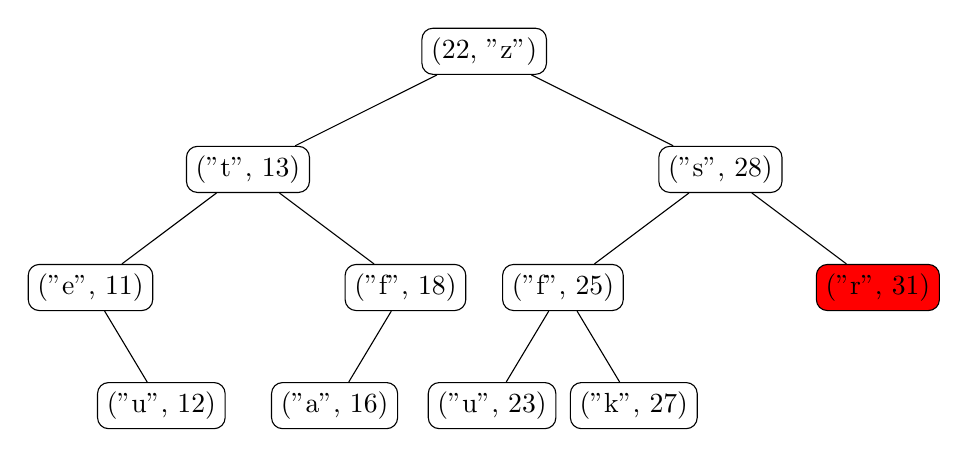
\begin{tikzpicture}[level distance = 15mm]
  \tikzstyle{level 1}=[sibling distance =6cm]
  \tikzstyle{level 2}=[sibling distance =4cm]
  \tikzstyle{level 3}=[sibling distance =18mm]
  \tikzstyle{every node}=[rectangle,draw, rounded corners]
  \node {($22$, "z")}
   child {node{("t", $13$)}
           child {node{("e", 11)}
                  child [missing]
                  child {node{("u", 12)}}
                 }
           child {node{("f", 18)}
                  child {node{("a", 16)}}
                  child [missing]
                 }
        }
  child {node{("s", 28)}
           child {node{("f", 25)}
                  child {node{("u", 23)}}
                  child {node{("k", 27)}}
                 }
           child {node[fill=red]{("r", 31)}}
        };
\end{tikzpicture}
\caption{Élément de priorité maximale}
\end{figure*}
%----------------------------------------------------------------
On peut donc écrire
%----------------------------------------------------------------
\begin{code}{Fonctions concernant l'élément de priorité maximale}
let premier fp = 
   let rec aux arbre = 
      match arbre with
      |Vide -> failwith "La file est vide"
      |Noeud(_, (x, k), Vide) -> x
      |Noeud(_, _, d) -> aux d in
   aux fp.contenu;;

let enlever fp =
   let rec aux arbre = 
      match arbre with
      |Vide -> failwith "La file est vide"
      |Noeud(g, _, Vide) -> g
      |Noeud(g, n, d) -> Noeud(g, n, aux d) in
   fp.contenu <- aux fp.contenu;; 
\end{code}
%----------------------------------------------------------------
La complexité de \type{ajouter}, \type{premier} et \type{enlever} est de l'ordre de la hauteur de l'arbre : en moyenne on peut compter sur une complexité en ${\cal O}\bigl(\log_2(n)\bigr)$ mais elle peut atteindre $n$ dans le pire des cas si on ne maintient pas un arbre équilibré.
La structure d'arbre est persistante, cela implique que la complexité spatiale peut devenir importante : à chaque ajout et retrait on crée un nombre de nœuds de l'ordre de la hauteur.

\medskip

Pour supprimer ou changer une priorité, on a besoin de repérer un élément par sa valeur et non sa priorité. La complexité sera alors celle d'un parcours d'arbre, linéaire en la taille et non en la hauteur.
%----------------------------------------------------------------
%----------------------------------------------------------------
\begin{exo}{Suppression}{}
Écrire les fonctions \type{supprimer} et \type{changerPrio} dans le cas de cette implémentation.
%----------------------------------------------------------------
\reponse
%----------------------------------------------------------------
\begin{ocaml}
let rec supprimer x fp =
   let rec oter arbre =
      match arbre with
      |Vide -> Vide
      |(y, p)::reste when y = x ->  suppressionRacine  arbre
      |Noeud(g, r, d) -> Noeud(oter g, r, oter d) in
    fp.contenu <- oter fp.contenu;;

let changerPrio x p fp =
   supprimer x fp;
   ajouter x p fp;;
\end{ocaml}
\end{exo}
%----------------------------------------------------------------
%----------------------------------------------------------------
%----------------------------------------------------------------
\newpage
%----------------------------------------------------------------
\section{Tas}
%----------------------------------------------------------------
%----------------------------------------------------------------
Nous allons maintenant définir une structure d'arbre moins structurée que celle d'arbre binaire de recherche mais suffisante pour gérer les priorités.
%----------------------------------------------------------------
%----------------------------------------------------------------
\subsection{Rappel : arbres quasi-complets à gauche}
%----------------------------------------------------------------
%----------------------------------------------------------------
\begin{defin}{Complétude d'arbres binaires}{}
Un arbre binaire de hauteur $h$ est 
\begin{description}
\item[complet] si toutes les feuilles sont de profondeur $h+1$,
\item[quasi-complet] si toutes les feuilles sont de profondeur $h$ ou $h+1$,
\item[quasi-complet à gauche] s'il est quasi-complet et si, de plus, les nœuds de profondeur $h$ sont tous situés à gauche.
\end{description}
\end{defin}
%----------------------------------------------------------------
On a vu qu'alors le nombre de nœuds de profondeur $k$ est $2^k$ pour tout $k<h$.

On en déduit que la taille $n$ de l'arbre vérifie $2^h\le n < 2^{h+1}$.
%----------------------------------------------------------------
\begin{figure*}[ht]
\centering
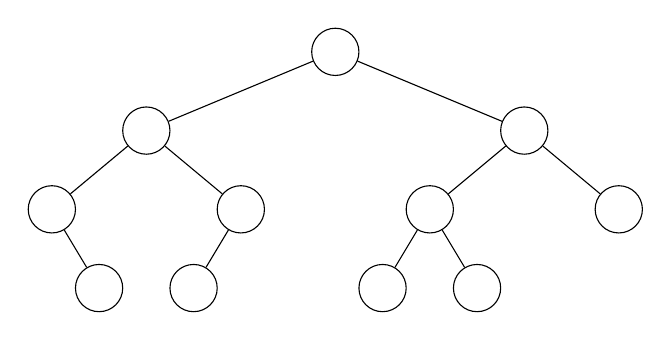
\begin{tikzpicture}[arbre3=6mm]
  \node {}
   child {node{}
           child {node{}
                  child [missing]
                  child {node{}}
                 }
           child {node{ }
                  child {node{}}
                  child [missing]
                 }
        }
  child {node{}
           child {node{}
                  child {node{}}
                  child {node{}}
                 }
           child {node{}}
        };
\end{tikzpicture}
\caption{Arbre quasi-complet}

\medskip

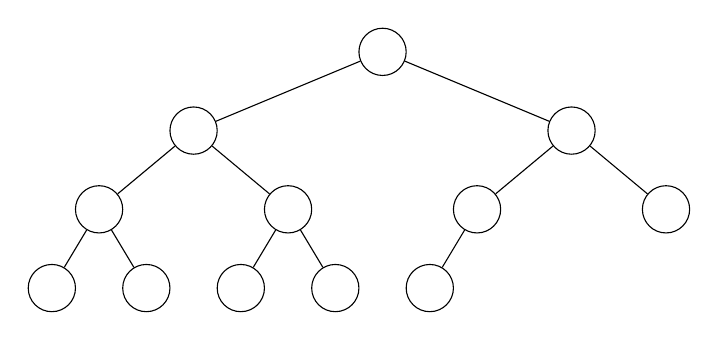
\begin{tikzpicture}[arbre3=6mm]
  \node {}
   child {node{}
          child {node{}
                 child {node{}}
                 child {node{}}
                 }
           child {node{}
                  child {node{}}
                  child {node{}}
                 }
         }
  child {node{}
         child {node{}
                child {node{}}
                child [missing]
               }
         child {node{}}
        };
\end{tikzpicture}
\caption{Arbre quasi-complet à gauche}
\end{figure*}
%----------------------------------------------------------------
%----------------------------------------------------------------
\begin{exo}{Caractérisation des arbres complets}{}
Écrire une fonction \type{complet : 'a arbre -> bool} qui renvoie \type{true} si et seulement si l'arbre est complet.
%----------------------------------------------------------------
\reponse
%----------------------------------------------------------------
Un arbre est complet s'il est vide ou si ses deux fils sont complets de même hauteur.

On va écrire une fonction qui renvoie le booléen et la hauteur.
\begin{ocaml}
let rec complet_h arbre =
   match arbre with
   |Vide -> true, -1
   |Noeud(g, _, d) -> let cg, hg = aux g in
                      let cd, hd = aux d in
                      hg = hd && cg && cd, (max hg hd) + 1;;
                      
let complet arbre = fst (complet_h arbre);;
\end{ocaml}
\end{exo}
%----------------------------------------------------------------
%----------------------------------------------------------------
\begin{exo}{Caractérisation des arbres quasi-complets à gauche}{}

Donner une caractérisation (récursive) d'un arbre quasi-complet à gauche en fonction de ses fils droit et gauche (quasi-complets à gauche ou complets) ; la hauteur intervient.

En déduire une fonction \type{qcg : 'a arbre -> bool} qui renvoie \type{true} si et seulement si l'arbre est quasi-complet à gauche mais non complet.
%----------------------------------------------------------------
\reponse
%----------------------------------------------------------------
Un arbre de hauteur $h$ est quasi-complet à gauche si et seulement si
\begin{itemize}
    \item il est non vide, l'arbre vide est complet
    \item son fils gauche est quasi-complet à gauche de hauteur $h-1$ et son fils droit est complet de hauteur $h-2$
    \item son fils gauche est complet de hauteur $h-1$ et son fils droit est complet de hauteur $h-2$
    \item son fils gauche est complet de hauteur $h-1$ et son fils droit est quasi-complet à gauche de hauteur $h-1$
\end{itemize}

Pour gérer les différents cas on peut définir un nouveau type :
\begin{ocaml}
type completude = C of int | QCG of int | Non;;
\end{ocaml}
\type{C h} caractérise un arbre complet de hauteur $h$ ($h\ge -1$), \type{QCG h} caractérise un arbre quasi-complet à gauche de hauteur $h$ ($h\ge 1$) et \type{Non} caractérise les autres arbres.

\begin{ocaml}
let rec typeC arbre =
   match arbre with
   |Vide -> C (-1)
   |Noeud(Vide, x, Vide) -> C 0
   |Noeud(g, x, d) -> begin match typeC g, typeC d with
                      |C hg, C hd when hg = hd -> C (hg + 1)
                      |C hg, C hd when hg = hd + 1 -> QCG (hg +1)
                      |C hg, QCG hd when hg = hd -> QCG (hg +1)
                      |QCG hg, C hd when hg = hd + 1 -> QCG (hg +1)
                      |_ -> Non end;;
let qcg arbre =
   match typeC arbre with
   |QCG h -> true
   |_ -> false;;
\end{ocaml}
\end{exo}
%----------------------------------------------------------------
\newpage
%----------------------------------------------------------------
\subsection{Décroissance verticale}
%----------------------------------------------------------------
%----------------------------------------------------------------
\begin{defin}{Arbres décroissants}{}
Un arbre décroissant est un arbre binaire dont les nœuds possèdent une clé et tel que la clé d'un nœud est toujours inférieure à celle de son père.
\end{defin}
%----------------------------------------------------------------

On a donc remplacé la croissance des clé "en largeur" des arbres binaires de recherche par une croissance du bas vers le haut moins contraignante.
%----------------------------------------------------------------
\begin{figure*}[ht]
\centering
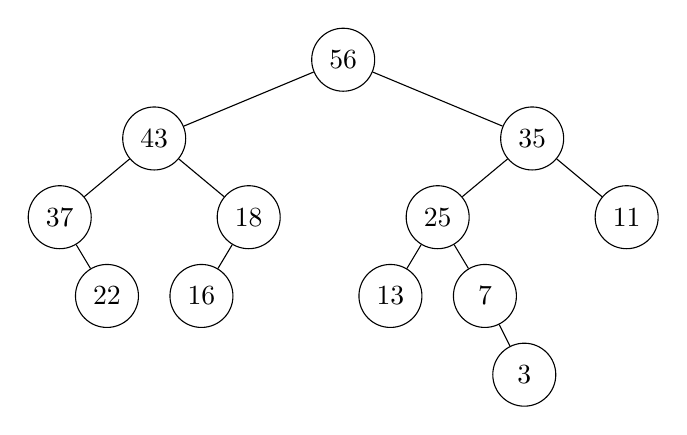
\begin{tikzpicture}[arbre3]
  \node {$56$}
  child {node{$43$}
          child {node{$37$}
                 child [missing]
                 child {node{$22$}}
                }
          child {node{$18$}
                 child {node{$16$}}
                 child [missing]
                }
         }
  child {node{$35$} 
          child {node{$25$}
          child {node{$13$}}
                 child {node{$7$}
                        child [missing]
                        child {node{$3$}}
                        }
                }
          child {node{$11$}}
         };
\end{tikzpicture}
\caption{Un arbre décroissant}
\end{figure*}
%----------------------------------------------------------------
\begin{defin}{Tas}{}
	Un tas est un arbre décroissant quasi-complet à gauche.
\end{defin}
%----------------------------------------------------------------
\begin{figure*}[ht]
\centering
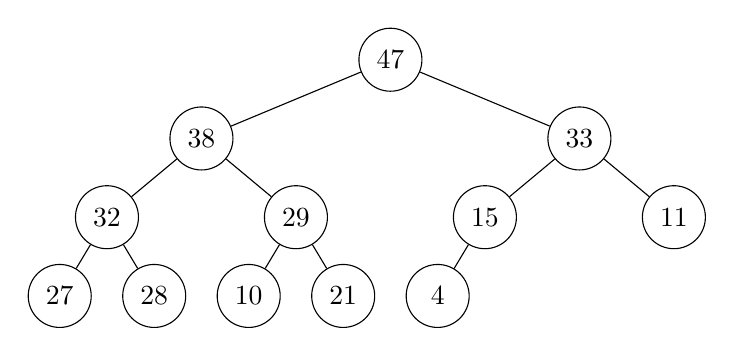
\begin{tikzpicture}[arbre3]
  \node {$47$}
  child {node{$38$}
          child {node{$32$}
                 child {node{$27$}}
                 child {node{$28$}}
                }
          child {node{$29$}
                 child {node{$10$}}
                 child {node{$21$}}
                }
         }
  child {node{$33$} 
          child {node{$15$}
                 child {node{$4$}}
                 child [missing]
                }
          child {node{$11$}}
         };
\end{tikzpicture}
\caption{Le tas $t_0$}
\end{figure*}
%----------------------------------------------------------------
\newpage
%----------------------------------------------------------------
\subsection{Opérations abstraites}
%----------------------------------------------------------------
%----------------------------------------------------------------
On suppose qu'en plus du type de données d'arbre on dispose de fonctions qui permettent 
\begin{itemize}
    \item de trouver le père d'un nœud (distinct de la racine),
    \item de parvenir au dernier nœud non vide (dans le parcours en largeur),
    \item de parvenir au premier nœud vide (à droite du précédent).
\end{itemize}
Dans $t_0$, le dernier nœud non vide a la valeur $4$.
%----------------------------------------------------------------
\subsubsection{Ajouter}
%----------------------------------------------------------------
	Pour ajouter un élément commence par l'ajouter à la position suivante dans l'ordre du parcours en largeur puis on le remonte tant que sa valeur est supérieure à celle de son père. 
	
	On va ajouter 42 à $t_0$.
%----------------------------------------------------------------
\begin{figure*}[ht]
\centering
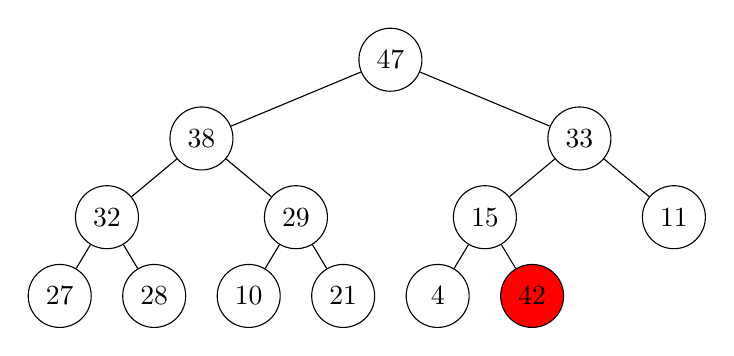
\begin{tikzpicture}[arbre3]
  \node {$47$}
  child {node{$38$}
          child {node{$32$}
                 child {node{$27$}}
                 child {node{$28$}}
                }
          child {node{$29$}
                 child {node{$10$}}
                 child {node{$21$}}
                }
         }
  child {node{$33$} 
          child {node{$15$}
                 child {node{$4$}}
                 child {node[fill = red]{$42$}}
                }
          child {node{$11$}}
         };
\end{tikzpicture}
\caption{Première étape : placement de 42 à la première feuille vide}
\medskip
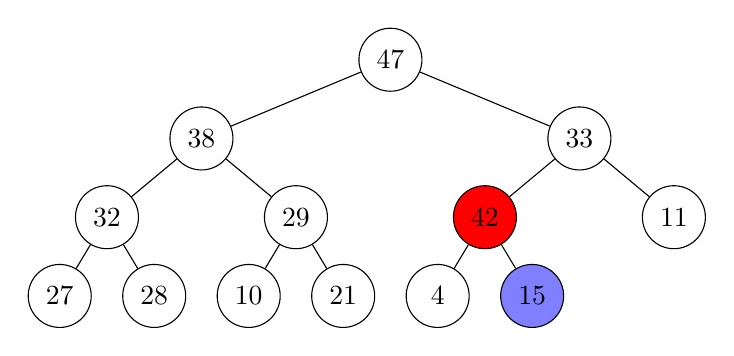
\begin{tikzpicture}[arbre3]
  \node {$47$}
  child {node{$38$}
          child {node{$32$}
                 child {node{$27$}}
                 child {node{$28$}}
                }
          child {node{$29$}
                 child {node{$10$}}
                 child {node{$21$}}
                }
         }
  child {node{$33$} 
          child {node[fill = red]{$42$}
                 child {node{$4$}}
                 child {node[fill = blue!50]{$15$}}
                }
          child {node{$11$}}
         };
\end{tikzpicture}
\medskip
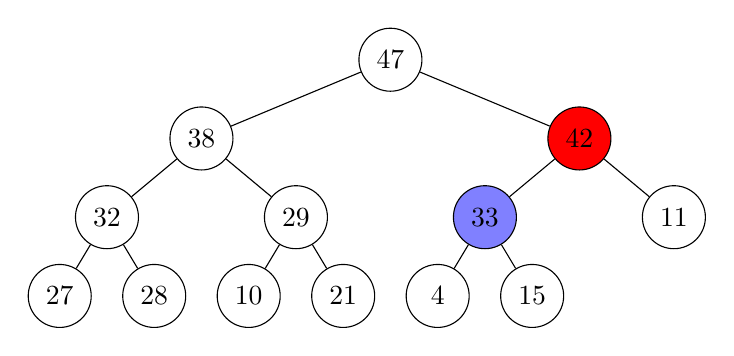
\begin{tikzpicture}[arbre3]
  \node {$47$}
  child {node{$38$}
          child {node{$32$}
                 child {node{$27$}}
                 child {node{$28$}}
                }
          child {node{$29$}
                 child {node{$10$}}
                 child {node{$21$}}
                }
         }
  child {node[fill = red]{$42$}
          child {node[fill = blue!50]{$33$}
                 child {node{$4$}}
                 child {node{$15$}}
                }
          child {node{$11$}}
         };
\end{tikzpicture}
\caption{Deuxième étape : échanges de 42 avec un père plus petit}
\end{figure*}
%----------------------------------------------------------------
\newpage
%----------------------------------------------------------------
\subsubsection{Enlever}
%----------------------------------------------------------------
Pour enlever l'élément maximum d'un tas on procède comme dans le cas de l'ajout.
\begin{itemize}
    \item On modifie l'ensemble des élément de l'arbre en maintenant la structure d'arbre quasi-complet à gauche ; ici on va remplacer l'élément à la racine par la dernière valeur dans un nœud, en supprimant aussi le dernier nœud.
    \item On reconstitue la structure croissante : ici on va descendre l'élément tant qu'il est inférieur à l'un de ses fils en le remplaçant par le plus grand de ses fils.
\end{itemize}

%----------------------------------------------------------------
\begin{figure*}[ht]
\centering
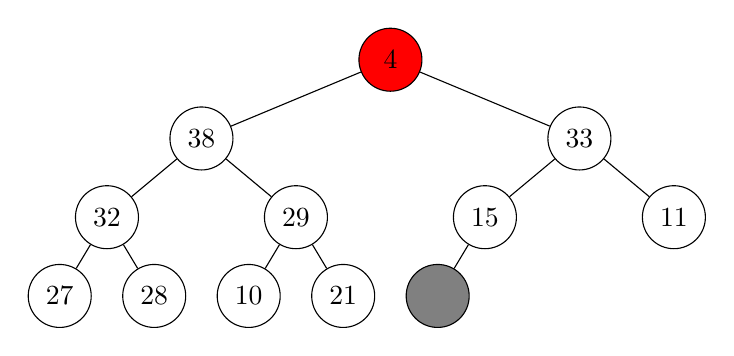
\begin{tikzpicture}[arbre3]
  \node[fill=red] {$4$}
  child {node{$38$}
          child {node{$32$}
                 child {node{$27$}}
                 child {node{$28$}}
                }
          child {node{$29$}
                 child {node{$10$}}
                 child {node{$21$}}
                }
         }
  child {node{$33$} 
          child {node{$15$}
                 child {node[fill=gray]{}}
                 child [missing]
                }
          child {node{$11$}}
         };
\end{tikzpicture}
% \begin{tikzpicture}
% \graph [binary tree layout, nodes={circle, draw, minimum size =8mm, level distance = 10mm}]
% {4[fill = red] -- {38 -- {32 -- {27, 28},
%                           29 -- {10, 21}
%                          },
%                   33 -- {15 -- ""[fill = gray], 11}
%                   }
% };
% \end{tikzpicture}
\caption{Première étape : remplacement de 47 par 4 dans $t_0$}
\medskip
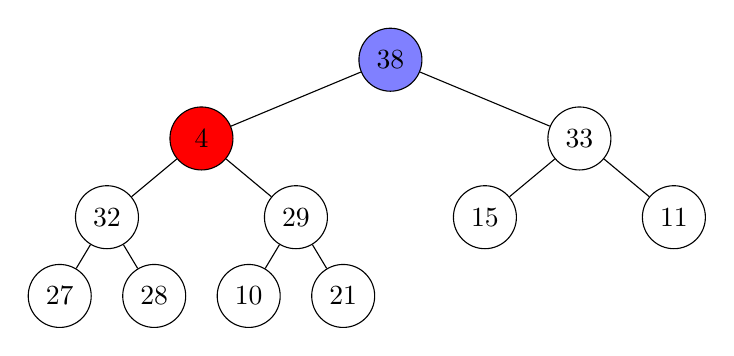
\begin{tikzpicture}[arbre3]
  \node[fill = blue!50] {$38$}
  child {node[fill=red]{$4$}
          child {node{$32$}
                 child {node{$27$}}
                 child {node{$28$}}
                }
          child {node{$29$}
                 child {node{$10$}}
                 child {node{$21$}}
                }
         }
  child {node{$33$} 
          child {node{$15$}}
          child {node{$11$}}
         };
\end{tikzpicture}
\medskip
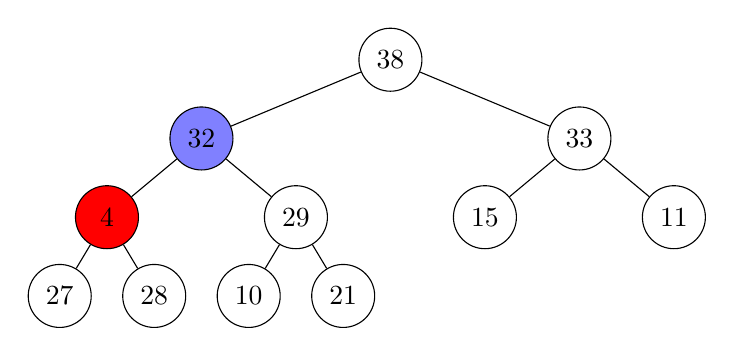
\begin{tikzpicture}[arbre3]
  \node{$38$}
  child {node[fill = blue!50]{$32$}
          child {node[fill=red]{$4$}
                 child {node{$27$}}
                 child {node{$28$}}
                }
          child {node{$29$}
                 child {node{$10$}}
                 child {node{$21$}}
                }
         }
  child {node{$33$} 
          child {node{$15$}}
          child {node{$11$}}
         };
\end{tikzpicture}
\medskip
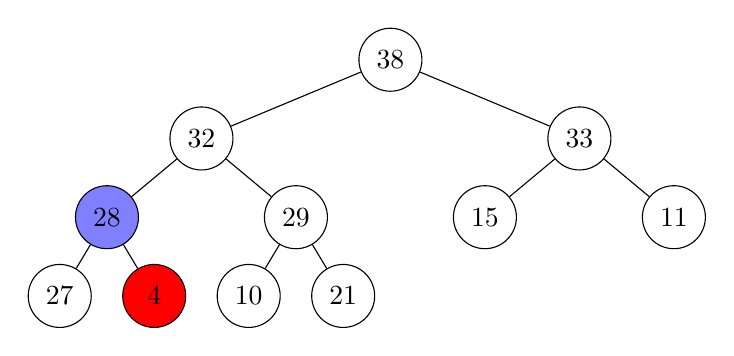
\begin{tikzpicture}[arbre3]
  \node{$38$}
  child {node{$32$}
          child {node[fill = blue!50]{$28$}
                 child {node{$27$}}
                 child {node[fill=red]{$4$}}
                }
          child {node{$29$}
                 child {node{$10$}}
                 child {node{$21$}}
                }
         }
  child {node{$33$} 
          child {node{$15$}}
          child {node{$11$}}
         };
\end{tikzpicture}
\caption{Deuxième étape : échanges de 4 avec son plus grand fils}
\end{figure*}
%----------------------------------------------------------------
\newpage
%----------------------------------------------------------------
\subsection{Réalisation par tableaux}
%----------------------------------------------------------------
Il est possible de réaliser les constructions ci-dessus avec des arbres : la difficulté technique est dans l'accès aux dernier nœud ou à la première feuille vide, voir l'exercice . Cependant le problème de l'occupation en mémoire demeure : chaque opération crée des nouveaux nœuds, le long d'une branche avec un ordre de grandeur de $\log_2(n)$.

Pour diminuer cette complexité spatiale, on va utiliser un type de donnée impératif pour stocker les valeurs des nœuds : un tableau. En effet le parcours en largeur d'un arbre quasi-complet à gauche fournit une bijection entre les nœuds et un tableau.

%----------------------------------------------------------------
\begin{figure*}[ht]
\centering
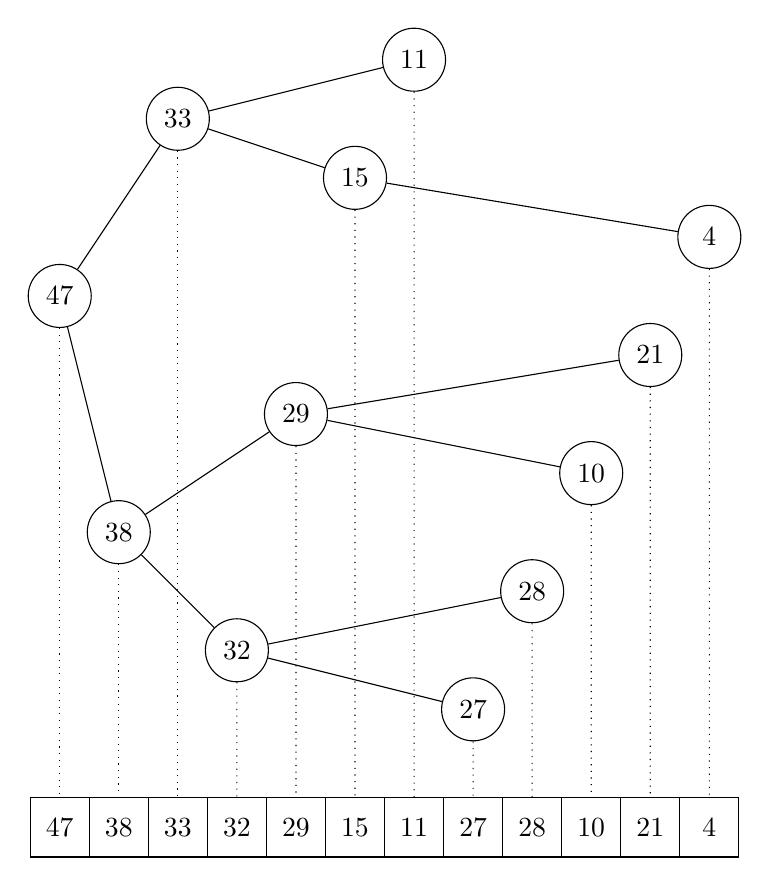
\begin{tikzpicture}[scale = 0.75, every node/.style={minimum size=0.8cm, draw}]
\foreach \n/\x/\y in {47/0/0, 38/1/-4, 33/2/3, 32/3/-6, 29/4/-2, 15/5/2, 11/6/4, 27/7/-7, 28/8/-5, 10/9/-3, 21/10/-1, 4/11/1}
   {\node[circle] (\n) at (\x, \y) {\n};
    \node[minimum size = 0.75cm] (t\n) at (\x,-9) {\n};
    \draw[dotted] (\n) -- (t\n);};
\foreach \p\f in {47/38, 47/33, 38/32, 38/29, 33/15, 33/11, 32/27, 32/28, 29/10, 29/21, 15/4}
   \draw (\p) --(\f);
\end{tikzpicture}
\caption{Parcours en largeur de $t_0$}
\end{figure*}

%----------------------------------------------------------------


Comme la structure de tableau n'est pas dynamique, le nombre d'éléments est fixé, on va inclure le tableau utilisé dans un tableau assez grand pour pouvoir contenir le nombre maximal d'éléments. Bien entendu il est difficile de prévoir et il y a un risque de débordement.On doit alors maintenir un entier qui sera la taille de la file.

\medskip

On a besoin d'une fonction de clé pour comparer les valeurs d'un tas. On va traiter directement le cas des files de priorité.
\begin{ocaml}
let nMax = 100;;

type 'a tas = {mutable taille : int; 
                        arbre : 'a array};;
                        
type 'a fdp = ('a * int) tas;;

let cle = snd;;
\end{ocaml}
%----------------------------------------------------------------
Les fonctions simples sont en temps constant
%----------------------------------------------------------------
\begin{ocaml}
let fpVide a =
  {taille = 0; arbre = Array.make nMax (a, 0) };;

let estVide t =  
  t.taille = 0;;

let premier t = 
  fst t.arbre.(0);;
\end{ocaml}
%----------------------------------------------------------------
On aura besoin de la traditionnelle fonction d'échange :
%----------------------------------------------------------------
\begin{ocaml}
let echange tab i j =
      let temp = tab.(i) in
      tab.(i) <- tab.(j);
      tab.(j) <- temp;;
\end{ocaml}
%----------------------------------------------------------------

Pour les fonctions \type{ajouter} et \type{enlever} on a besoin de connaître l'indice du père d'un nœud ou les indices de ses fils.
\begin{thm}{Numérotation des fils}{}
Avec la numérotation du tableau de 0 à $n-1$, le père du nœud d'indice $i$ a pour indice $(i-1)/2$ et ses fils guache et droit ont pour indices $2i +1$ et $2i+2$ respectivement.
\end{thm}

L'ajout se fait comme indiqué ci-dessus avec une fonction auxiliaire pour effectuer la remontée.
%----------------------------------------------------------------
\begin{code}{Ajout d'un élément}
let rec remonter n t =
   if n > 0
      then let m = (n-1)/2 in
         if (cle t.(m)) < (cle t.(n))
         then (echange t m n; remonter m t);;

let ajouter_tas x tas  =
  let n = tas.taille in
    tas.arbre.(n) <- x;
    tas.taille <- n + 1;
    remonter n t.arbre;;
    
let ajouter x p file = ajouter_tas (x, p) file;;
\end{code}
%----------------------------------------------------------------
Pour la fonction \type{enlever} on a vu qu'il faut redescendre les éléments et effectuant un échange avec le fils de priorité maximale. 

On commence par rechercher ce fils. Comme il peut ne pas exister de fils on va renvoyer un type optionnel (\type{Some/None}) qui permet de gérer l'absence de réponse. Le dernier indice possible est $n-1$ si $n$ est la taille, un nœud d'indice $k$ peut admettre des fils d'indice $2k+1$ et $2k+2$.

Le nombre de fils de $k$ est donc 0 pour $n-1 < 2k+1$, 1 pour $n-1=2k+1$ et 2 pour $n-1 > 2k+1$.
%----------------------------------------------------------------
\begin{code}{Retrait du terme de priorité maximale}
let filsGrand k t n =
   if n <= 2*k + 1 
   then None
   else if n = 2*k + 2  
        then Some (2*k + 1)
        else if (cle t.(2*k+1)) < (cle t.(2*k+2))
             then Some (2*k + 2) else Some (2*k + 1);;  

let rec descendre k t n =
   match filsGrand k t n with
   |Some p when (cle t.(p)) > (cle t.(k))
       -> (echange t k p; descendre p t n)
   |_ -> ();;

let enlever_tas tas =
   let n  = tas.taille -1 in
   let t  = tas.arbre in
   echange t 0 n;
   tas.taille <- n;
   descendre 0 t n;;
  
let enlever file = fst (enlever_tas file);;
\end{code}

%----------------------------------------------------------------

Les complexités des fonctions \type{ajouter} et \type{enlever} sont celles de  \type{monter} et \type{descendre}. Dans ces dernières on fait un nombre fini d'opérations et on appelle récursivement avec un nœud de profondeur modifiée de 1 ou $-1$ donc les complexités sont en ${\cal O}(h)$ où $h$ est la hauteur. Comme l'arbre est équilibré on en déduit
%----------------------------------------------------------------
\begin{thm}{Complexités dans un tas}{}
Les complexités des fonctions \type{ajouter} et \type{enlever} sont en ${\cal O}\bigl(\ln(n)\bigr)$ où $n$ est la taille du tas. Les autres fonctions sont de complexité constante.
\end{thm}
%----------------------------------------------------------------
%----------------------------------------------------------------
\subsection{Exercices}
%----------------------------------------------------------------
%----------------------------------------------------------------
\begin{exo}{Test de tas}{}
Écrire une fonction \type{estTas t p} qui teste si les valeurs d'un tableau comprises ont des indices compris entre 0 à $p-1$ forment un tas.
%----------------------------------------------------------------
\reponse
%----------------------------------------------------------------
Un tableau est un tas si tous les fils ont une clé supérieure à celle de leur père. Plutôt que tester les fils d'un nœud, il faudrait s'assurer de leur existence, on va tester le père de chaque nœud.

\begin{ocaml}
let estTas t p =
   let valide = ref true in
      for i = 1 to (p-1) do
      if  t.(i) >= t.((i-1)/2) then valide := false done;
   !valide;;
\end{ocaml}
\end{exo}
%----------------------------------------------------------------
%----------------------------------------------------------------
\begin{exo}{Suppression dans un tas}{}
 Écrire la fonction \type{suprimer}. Quelle est sa complexité ?
%----------------------------------------------------------------
\reponse
%----------------------------------------------------------------
On n'a pas d'algorithme efficace pour retrouver un élément, la complexité est linéaire en la taille.
\begin{ocaml}
let supprimer x tas =
   let n  = tas.taille in
   let t = tas.arbre in
   let i = ref 0 in
   while !i < n && fst t.(i) <> x do  incr i done;
   if !i < n
   then begin t.(i) <- t.(n);
              tas.taille <- n-1 end;;
\end{ocaml}
\end{exo}
%----------------------------------------------------------------
%----------------------------------------------------------------
\section{Heapsort}
%----------------------------------------------------------------
%----------------------------------------------------------------
Dès qu'on a une structure de file de priorité on peut l'utiliser pour réaliser un tri.

On remplit une file à partir d'une file vide vide en ajoutant un à un les éléments d'un tableau (ou une liste). On retire ensuite les éléments un à un en formant un tableau : celui-ci sera trié.

La complexité du tri est alors un ${\cal O}\bigl(n(a+b)\bigr)$ où $a$ et $b$ sont les complexité respective de l'ajout et du retrait d'un élément.

Comme on sait que la complexité d'un tri par comparaisons est au moins un ${\cal O}\bigl(n\log(n)\bigr)$ on voit qu'une au moins des deux opérations ci-dessus doit être en ${\cal O}\bigl(\log(n)\bigr)$.

On peut considérer que le tri par insertion correspond à ce schéma avec une file de priorité implémentée par un tableau trié tandis que tri par sélection correspond à une file de priorité implémentée par un tableau non trié. On retrouve bien une complexité en ${\cal O}\bigl(n^2\bigr)$ car l'une des deux opérations est de complexité linéaire.

L'implémentation par un tas donne un tri de complexité asymptotique optimale.

\medskip

Comme dans le cas des tris par insertions on ne va pas utiliser les fonction du type abstrait : on va travailler directement sur la structure de données.

\medskip

Si \type{t} est un tableau, il peut être vu comme un arbre quasi-complet à gauche mais cet arbre n'est pas, en général, décroissant. Comme les éléments sont déjà présents dans le tableau on peut le transformer en tas en ajoutant les éléments depuis l'indice 0 vers l'indice $n-1$ : pour chaque $i$ on remonte \type{t.(i)}  dans le tas formé par les éléments de 0 à $i-1$ qui forment un tas. La clé ici est simplement la valeur.
%----------------------------------------------------------------
\begin{ocaml}
let cle x = x;;
\end{ocaml}

%----------------------------------------------------------------
%----------------------------------------------------------------
\begin{exo}{Création d'un tas}{}
En utilisant uniquement la fonction \type{remonter}, écrire une fonction qui transforme \type{t} en un tas.

Quelle en est la complexité ?
%----------------------------------------------------------------
\reponse
%----------------------------------------------------------------
\begin{ocaml}
let mettreEnTas t =
  let n = Array.length t in
  let tas = {taille = n; arbre = t} in
  for i = 0 to (n-1) do remonter i tas done;
  tas;;
\end{ocaml}

La complexité est majorée par $\displaystyle \sum_{i=1}^{n-1} \lfloor\log_2(i+1)\rfloor$ : c'est un ${\cal O}\bigl(n\log(n)\bigr)$.
\end{exo}
%----------------------------------------------------------------
%----------------------------------------------------------------
Lorsqu'on en enlève tous les éléments d'un tas un par un ceux-ci sont placés dans les emplacements depuis la position $n-1$ vers la gauche. Les $n$ premier termes du tableau sont alors triés car le premier élément retiré est celui de priorité maximale.
%----------------------------------------------------------------
%----------------------------------------------------------------
\begin{exo}{Tri d'un tas}{}
En vous inspirant de cette remarque écrire une fonction (sans résultat) qui trie un tableau en place.
%----------------------------------------------------------------
\reponse
%----------------------------------------------------------------

\begin{ocaml}
let triParTas t =
  let tas = mettreEnTas t in
  let n = tas.taille in
  for i = 0 to (n-1) do enlever tas done;;
\end{ocaml}

Le tableau \type{t} est alors trié.

\begin{ocaml}
let t = [|5; 12; 9; 1; 8; 13; 4|];;
triParTas t;;
t;;

# - : int array = [|1; 4; 5; 8; 9; 12; 13|]
\end{ocaml}
La complexité est toujours un ${\cal O}\bigl(n\log(n)\bigr)$.
\end{exo}
%----------------------------------------------------------------
%----------------------------------------------------------------
La première étape peut être améliorée en construisant le tas non pas du haut vers le bas  mais en construisant des tas depuis le bas. Initialement les nœuds forment des tas de taille 1 juxtaposés.

On va former des tas de plus en plus gros en descendant les pères pour former un tas avec leurs fils qui eux-mêmes des tas. Pour cela on doit travailler depuis le dernier père (dans l'ordre des indices) vers le premier.

Dans l'exemple suivant on part de \type{[|15; 22; 29; 11; 18; 31|]} ; les nœuds colorés forment une forêt de tas, à la fin il ne restera qu'un tas unique.
%----------------------------------------------------------------
\begin{center}
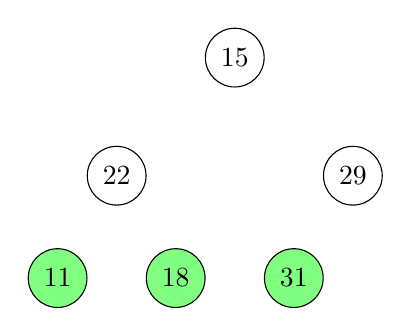
\begin{tikzpicture}
\tikzstyle{every node}=[circle,draw]
\node at (0,0) (r) {15};
\node at (-1.5,-1.5) (fg) {22};
\node at (1.5,-1.5) (fd) {29};
\node[fill = green!50] at (-2.25,-2.8) (fgg) {11};
\node[fill = green!50] at (-0.75,-2.8) (fgd) {18};
\node[fill = green!50] at (0.75,-2.8) (fdg) {31};
\end{tikzpicture}
\text{On descend 29}
\quad
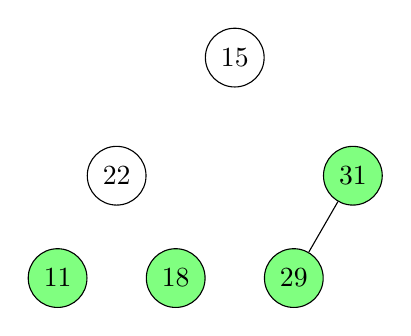
\begin{tikzpicture}
\tikzstyle{every node}=[circle,draw]
\node at (0,0) (r) {15};
\node at (-1.5,-1.5) (fg) {22};
\node[fill = green!50] at (1.5,-1.5) (fd) {31};
\node[fill = green!50] at (-2.25,-2.8) (fgg) {11};
\node[fill = green!50] at (-0.75,-2.8) (fgd) {18};
\node[fill = green!50] at (0.75,-2.8) (fdg) {29};
\draw (fdg) -- (fd);
\end{tikzpicture}
\end{center}

\medskip

\begin{center}
\text{22 ne bouge pas}
\quad
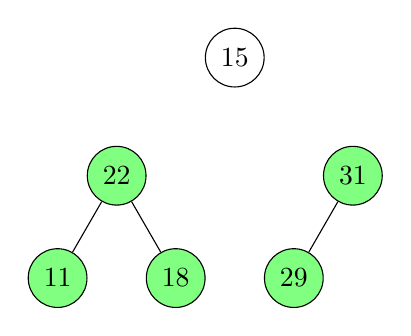
\begin{tikzpicture}
\tikzstyle{every node}=[circle,draw]
\node at (0,0) (r) {15};
\node[fill = green!50] at (-1.5,-1.5) (fg) {22};
\node[fill = green!50] at (1.5,-1.5) (fd) {31};
\node[fill = green!50] at (-2.25,-2.8) (fgg) {11};
\node[fill = green!50] at (-0.75,-2.8) (fgd) {18};
\node[fill = green!50] at (0.75,-2.8) (fdg) {29};
\draw (fdg) -- (fd);
\draw (fgg) -- (fg);
\draw (fgd) -- (fg);
\end{tikzpicture}
\end{center}

\medskip

\begin{center}
\text{15 descend à sa place}
\quad
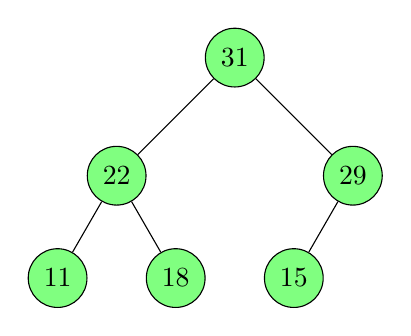
\begin{tikzpicture}
\tikzstyle{every node}=[circle,draw]
\node[fill = green!50] at (0,0) (r) {31};
\node[fill = green!50] at (-1.5,-1.5) (fg) {22};
\node[fill = green!50] at (1.5,-1.5) (fd) {29};
\node[fill = green!50] at (-2.25,-2.8) (fgg) {11};
\node[fill = green!50] at (-0.75,-2.8) (fgd) {18};
\node[fill = green!50] at (0.75,-2.8) (fdg) {15};
\draw (fdg) -- (fd);
\draw (fgg) -- (fg);
\draw (fgd) -- (fg);
\draw (fg) -- (r);
\draw (fd) -- (r);
\end{tikzpicture}
\end{center}
%----------------------------------------------------------------
%----------------------------------------------------------------
\begin{exo}{Une amélioration}{}

Écrire une fonction qui transforme \type{t} en un tas avec cette méthode

Quelle est sa complexité ?
%----------------------------------------------------------------
\reponse
%----------------------------------------------------------------

Le dernier fils admet \type{n-1} pour indice donc le dernier père admet \type{(n-2)/2} pour indice.
\begin{ocaml}
let mettreEnTas t =
  let n = Array.length t in
  let m = (n-2)/2 in
  let tas = {taille = n; arbre = t} in
  for i = 0 to m do descendre (m-i) tas done;
  tas;;
\end{ocaml}
Il y a $2^k$ nœuds de profondeur $k$ pour $k < h$, hauteur de l'arbre.

Pour chacun de ces nœuds la descente demande au plus $h-k$ étapes.

La complexité est donc majorée par $\displaystyle \sum_{k=0}^{h-1} (h-k)2^k$.

Si on pose $\displaystyle S_p = \sum_{k=0}^{p-1} (p-k)2^k$ on a

$\displaystyle S_{p+1} = \sum_{k=0}^{p} (p+1-k)2^k
=2^p + \sum_{k=0}^{p-1} \bigl((p-k)2^k +2^k\bigr)
=2^p + S_p + \sum_{k=0}^{p-1}2^k = 2.2^p+S_p -1$.

Comme on a $S_0=0$, on en déduit $\displaystyle S_p = \sum_{k=0}^{p-1} 2.2^k -1 = 2.(2^p-1)-n$.

Ainsi $S_h$ est majoré par $2.2^h - h - 2$ avec $2^h \le n < 2^{h+1}$ donc $S_h\le 2n$ : la complexité est un ${\cal O}(n)$.
\end{exo}
%----------------------------------------------------------------
%----------------------------------------------------------------
\section{Problème 1 : tableaux fonctionnels}
%----------------------------------------------------------------
On a vu qu'on pouvait réaliser un arbre (complet à gauche) par un tableau.

Nous nous intéressons ici au problème inverse : donner une implémentation d'un tableau sous la forme d'un arbre (persistant).

Un tableau peut être vu comme une fonction depuis un ensemble d'indices vers l'ensemble des valeurs. On considère la fonction suivante qui associe un nœud à un entier non nul.

\begin{ocaml}
let rec elt k arbre =
  match arbre with
  |Vide -> failwith "Element non defini"
  |Noeud(g,n,d) -> if k = 1 then n
                            else if k mod 2 = 0
                                 then elt (k/2) g else elt (k/2) d;;
\end{ocaml}

Dans le cas $n=15$ on accède ainsi aux nœuds de l'arbre complet de hauteur 3.

\begin{center}
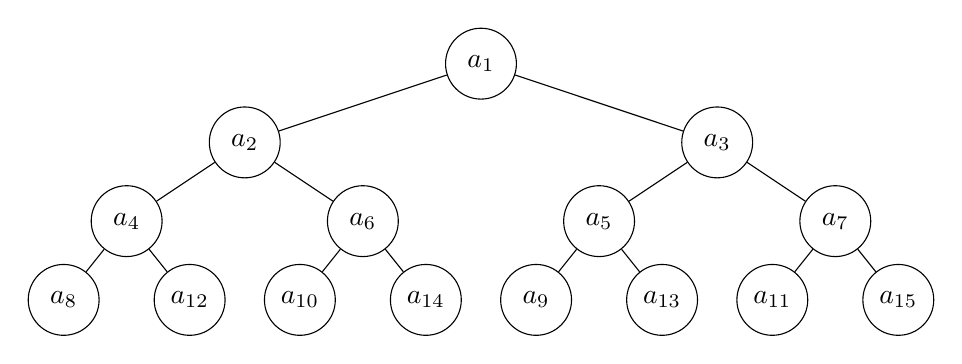
\begin{tikzpicture}[level distance =10mm,minimum size =9mm]
  \tikzstyle{level 1}=[sibling distance =6cm]
  \tikzstyle{level 2}=[sibling distance =3cm]
  \tikzstyle{level 3}=[sibling distance =16mm]
  \tikzstyle{every node}=[circle,draw]
  \node {$a_1$}
   child {node {$a_2$}
          child {node {$a_4$}
                 child {node {$a_8$}}
                 child {node {$a_{12}$}}
                }
          child {node {$a_6$}
                 child {node {$a_{10}$}}
                 child {node {$a_{14}$}}
                }
        }
   child {node {$a_3$}
          child {node {$a_5$}
                 child {node {$a_9$}}
                 child {node {$a_{13}$}}
                }
          child {node {$a_7$}
                 child {node {$a_{11}$}}
                 child {node {$a_{15}$}}
                }
        };
\end{tikzpicture}
\end{center}
On a ainsi défini une structure de tableau à accès presque constant qui a l'avantage d'être persistante (quand on change une valeur, l'ancien tableau peut exister encore) et qui, de plus, peut-être augmentée.
%----------------------------------------------------------------
%----------------------------------------------------------------
\begin{exo}{Tableaux fonctionnels}{}
\begin{itemize}
\item Écrire une fonction \type{change k x a} qui renvoie une nouvel arbre $a'$ tel que $a'_k =x$ et $a'_i = a_i$ pour $i\ne k$. Si la position n'était pas occupée mais si le père existe on ajoutera l'élément à sa place.

\item Écrire une fonction \type{creeTableau n x} qui renvoie un arbre de taille $n$ dont tous les éléments ont la valeur $x$.

\item Quelle est la complexité de \type{elt} et de \type{change} pour un tableau de taille $n$ ?

\end{itemize}
%----------------------------------------------------------------
\reponse
%----------------------------------------------------------------
\begin{itemize}
\item Pour transformer un élément il suffit de le chercher et de transformer le nœud :

\begin{ocaml}
let rec change k x arbre = 
  match arbre with
  |Vide -> if k = 1
           then Noeud(Vide, x, Vide)
           else failwith "Position non accessible"
  |Noeud(g,n,d) -> if k = 1
                   then Noeud(g,x,d)
                   else if k mod 2 = 0
                        then Noeud(change (k/2) x g ,n, d)
                        else Noeud(g, n, change (k/2) x d);;
\end{ocaml}
Comme suggéré par l'énoncé on autorise, si on parvient à un arbre vide, l'ajout d'un élément d'indice $k$ si l'élément d'indice $k/2$ est défini. En effet on ne peut appeler \type{change 1 x Vide} que depuis un arbre non vide\footnote{ou directement en voulant changer une valeur d'un tableau vide}.

\item On peut créer un tableau à partir du vide en ajoutant un-à-un tous les éléments grâce à la possibilité de la question précédente. Si on effectue cela récursivement on conserve en fait tous les tableaux intermédiaires. On va donc utiliser une boucle et modifier une variable référencée : cela permet au {\bf garbage collector} de libérer la place. 

\begin{ocaml}
let creeTableau n x =
  let a = ref Vide in
  for i = 1 to n do a := change i x !a done;
  !a;;
\end{ocaml}

On verra que les tableaux fonctionnels ont une structure équilibrée et que les fils sont similaires, le fils gauche ayant un terme de plus. On peut retrouver un algorithme récursif

\begin{ocaml}
let rec creeTableau n x =
  if n = 0
  then Vide
  else let k = (n-1)/2 in
       Noeud(creeTableau (n-1-k) x,x,creeTableau k x));;
\end{ocaml}

\item Comme indiqué ci-dessus, un tableau de taille $n\le 2^h-1$ est représenté par un arbre de hauteur $h$ donc les parcours de lecture ou de changement ont une complexité en $O(h)=O\bigl(\log(n)\bigr)$.
\end{itemize}
\end{exo}
%----------------------------------------------------------------
%----------------------------------------------------------------
On conserve la structure ci-dessus : on considère des arbres binaires de taille $n$ tels que les nœuds occupés correspondent aux indices de 1 à $n$. Ces arbres correspondent donc des tableaux de taille $n$ : on nommera {\bf arbres de Braun} de tels arbres.

\begin{center}
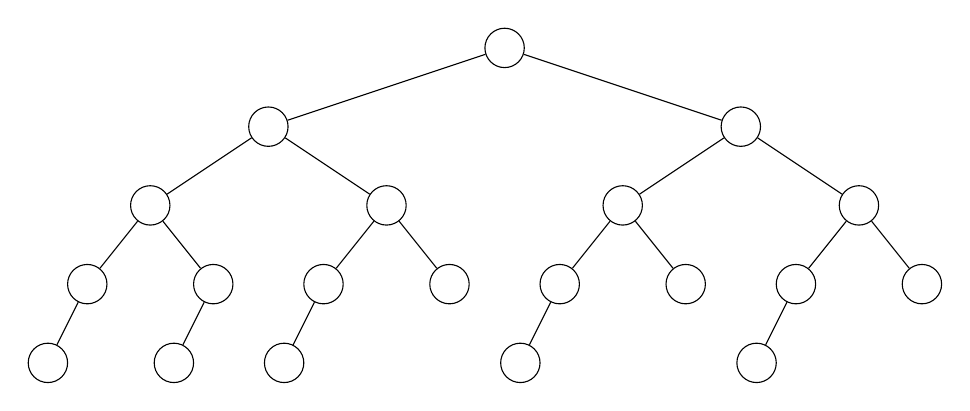
\begin{tikzpicture}[level distance =10mm,minimum size =5mm]
  \tikzstyle{level 1}=[sibling distance =6cm]
  \tikzstyle{level 2}=[sibling distance =3cm]
  \tikzstyle{level 3}=[sibling distance =16mm]
  \tikzstyle{level 4}=[sibling distance =10mm]
  \tikzstyle{every node}=[circle,draw]
  \node {}
   child {node {}
          child {node {}
                 child {node {}
                        child{node {}}
                        child {edge from parent[draw=none]}
                       }
                 child {node {}
                        child{node {}}
                        child {edge from parent[draw=none]}
                       }
                }
          child {node {}
                 child {node {}
                        child{node {}}
                        child {edge from parent[draw=none]}
                       }
                 child {node {}}
                }
        }
   child {node {}
          child {node {}
                 child {node {}
                        child{node {}}
                        child {edge from parent[draw=none]}
                       }
                 child {node {}}
                }
          child {node {}
                 child {node {}
                        child{node {}}
                        child {edge from parent[draw=none]}
                       }
                 child {node {}}
                }
        }
;
\end{tikzpicture}
\end{center}
%----------------------------------------------------------------
%----------------------------------------------------------------
\begin{exo}{Structure des arbres de Braun}{}
\type{t = Noeud(g,x,d)} est un arbre de Braun.
\begin{itemize}
\item Montrer que \type{g} et \type{d} sont des arbres de Braun.

\item Montrer que \type{taille g} = \type{taille d} ou  \type{taille g} = \type{taille d} +1.

\item Montrer que \type{hauteur g} = \type{hauteur d}  ou \type{hauteur g} = \type{hauteur d} +1.

\item Montrer que la feuille la plus à gauche est à la profondeur maximale.
\end{itemize}
%----------------------------------------------------------------
\reponse
%----------------------------------------------------------------
\begin{itemize}
\item L'arbre de gauche est défini par les positions $k$ pour $k$ pair. De plus, depuis la racine du fils gauche, on définit les positions à l'aide de $k/2$ ; on remplit donc un tableau fonctionnel avec les positions $2/2$, $4/2$, \dots, $n/2$. On construit ainsi un arbre de Braun.

De même pour le fils droit.

\item D'après la question précédente il y a $n/2=\lfloor \frac{n}{2} \rfloor$ nœuds dans le fils gauche.

La racine n'est dans aucun fils donc il y a  $n - 1 - \lfloor \frac{n}{2} \rfloor = \lceil \frac{n}{2} \rceil-1$ nœuds dans le fils droit.

On a $\lfloor \frac{n}{2} \rfloor \le \lceil \frac{n}{2} \rceil \le \lfloor \frac{n}{2} \rfloor + 1$ d'où le résultat.


\item Il n'y a qu'un arbre de Braun de taille $p$.

De plus l'arbre de taille $p+1$ est obtenu en ajoutant un élément.

Le fils gauche est ainsi égal au fils droit ou est obtenu en ajoutant un nœud ce qui ne peut augmenter la hauteur que de 1 au maximum.

\item La hauteur est atteinte pour le fils gauche d'après la troisième question.

Par récurrence on en déduit que la feuille la plus à gauche est à la hauteur maximale.
\end{itemize}
\end{exo}
%----------------------------------------------------------------
%----------------------------------------------------------------
On définit la fonction 
\begin{ocaml}
let rec ajouterBraun x t =
  match t with
  |Vide -> Noeud(Vide,x,Vide)
  |Noeud(g,y,d) -> Noeud(ajouterBraun x d,y,g);;
\end{ocaml}
%----------------------------------------------------------------
%----------------------------------------------------------------
\begin{exo}{Modification des arbres de Braun}{}
\begin{itemize}
\item Prouver que si \type{t} est un arbre de Braun alors \type{ajouter x t} est encore un arbre de Braun.
\item Comment enlever un élément en conservant la structure d'arbre de Braun ? 
\end{itemize}
%----------------------------------------------------------------
\reponse
%----------------------------------------------------------------
\begin{itemize}
\item On va montrer, par récurrence sur $n$ que la fonction \type{ajouterBraun x t} appliquée à un arbre qui représente un tableau fonctionnel d'indices de 1 à $n$ le transforme en un tableau fonctionnel d'indices de 1 à $n+1$.

\begin{itemize}
\item C'est évident pour $n=0$.
\item On suppose que cela est vrai pour tous les entiers $k\le n-1$ avec $n \ge 2$.

$t$ est un arbre de Braun de taille $n$, \type{t = Noeud(g,y,d)}, avec $g$ et $d$ de taille respectives $t_g$ et $t_d$.  

On note \type{t' = ajouterBraun x d} ; c'est, d'après l'hypothèse de récurrence, un arbre de Braun.

Si $d$ et $g$ ont la même taille $p$ alors $t'$ et $g$ sont des arbres de Braun de tailles respectives $p+1$ et $p$ donc \type{Noeud(t',y,g)} a la structure d'un arbre de Braun de taille $2p+1=n+1$.

De même si $g$ a un élément de plus que $d$.
\end{itemize}

\item La réciproque de "ajouter à droite puis inverser les fils" est "inverser les fils puis retrancher à droite" c'est-à-dire  "retrancher à gauche puis inverser les fils".

 La fonction renvoie la valeur enlevée en plus du nouvel arbre.

\begin{ocaml}[numbers=left]
let rec enleverBraun t =
  match t with
  |Vide -> failwith "Il n'y a rien à enlever"
  |Noeud(Vide,x,_) -> (x,Vide) (* Si g est vide alors d l'est aussi*)
  |Noeud(g,x,d) -> let (y,g') = enleverBraun g in
                   (y,Noeud(d,x,g'));;
\end{ocaml}
\end{itemize}
\end{exo}
%----------------------------------------------------------------
%----------------------------------------------------------------
Un {\bf tas de Braun} est un arbre de Braun décroissant.

%----------------------------------------------------------------
%----------------------------------------------------------------
\begin{exo}{Tas de Braun}{}
\begin{itemize}
\item Modifier la fonction \type{ajouterBraun} en préservant la structure de tas.

\item Comment enlever le plus petit élément en conservant la structure de tas de Braun ?
\end{itemize} 
%----------------------------------------------------------------
\reponse
%----------------------------------------------------------------
\begin{itemize}
\item On envoie vers le bas la plus petite clé :
\begin{ocaml}
let rec ajouterTasBraun x t =
  match t with
  |Vide -> Noeud(Vide,x,Vide)
  |Noeud(g,y,d) ->  if cle x < cle y
                    then Noeud(ajouterTasBraun x d,y,g)
                    else Noeud(ajouterTasBraun y d,x,g);;
\end{ocaml}

\item Pour enlever le plus petit élément, celui qui est à la racine, on peut

\begin{itemize}
\item enlever le dernier élément, en conservant sa valeur, 
\item le placer à la racine
\item le descendre en échangeant avec le plus grand de ses fils, récursivement.
\end{itemize}
On commence par écrire une fonction qui fait descendre un nœud de clé trop petite vers le bas de l'arbre. On supposera que l'arbre vérifie toutes les propriété à l'exception de la clé de la racine qui peut être trop petite.

\begin{ocaml}
let rec descendre t =
  match t with
  |Vide  -> t
  |Noeud(Vide,_,_) -> t
  |Noeud(Noeud(g,y,d),x,Vide)
   -> if x < y then t
               else Noeud(descendre(Noeud(g,x,d)),y,Vide)
  |Noeud(Noeud(g,y,d),x,Noeud(g',y',d'))
   -> if y < y'
      then (if x > y
            then Noeud(descendre(Noeud(g,x,d)),y,Noeud(g',y',d'))
            else t)
      else (if x > y'
            then Noeud(Noeud(g,y,d),y',descendre(Noeud(g',x,d')))
            else t);;
\end{ocaml}


Il suffit alors de remplacer la racine par le dernier terme et de faire descendre.

\begin{ocaml}
let resteTasBraun t =
  let (x,t') = enleverBraun t in
  match t' with
  |Vide -> Vide
  |Noeud(g,y,d) -> descendre(Noeud(g,x,d));; 
\end{ocaml}
\end{itemize}
\end{exo}
%----------------------------------------------------------------
%----------------------------------------------------------------
\section{Problème 2 : arbres gauchistes}
%----------------------------------------------------------------
%----------------------------------------------------------------
Nous avons implémenté les files d'attentes avec la structure de tas. Nous avons traduit la structure arborescente en tableau ce qui nous a fait perdre la persistance. Le problème ci-dessus a proposé une structure persistante, nous allons proposer une autre structure, persistante elle aussi, permettant d'implémenter une file d'attente avec des opérations de complexité garantie en $O\bigl(\log_2(n)\bigr)$.
%----------------------------------------------------------------
%----------------------------------------------------------------
\subsection{Rang vertical}
%----------------------------------------------------------------
%----------------------------------------------------------------
\begin{defin}{Rang vertical}{}
Dans un arbre le {\bf rang vertical} d'un nœud est la longueur de la plus courte branche (entre le nœud et une feuille) où on compte les nœuds. C'est la plus petite profondeur des fils vides.\end{defin}

Le rang vertical d'un tas est $h$, sa hauteur, sauf s'il est parfait, dans ce cas le rang est $h+1$.

On définit un nouveau type d'arbre binaire contenant le rang vertical :

\begin{ocaml}
type 'a arbreRV = VideRV 
                 |NoeudRV of int * 'a arbreRV * 'a * 'a arbreRV;;
\end{ocaml}

Un arbre avec un seul élément est de rang vertical 1 : \type{Noeud(1 ,Vide, x, Vide)}

%----------------------------------------------------------------
\begin{exo}{Première valeur}{}
Écrire une fonction \type{rangV : arbreRV -> int} qui renvoiela première valeur donnée dans \type{NoeudRV(k, g, r, d)} pour un n{\oe}ud et 0 sinon.
%----------------------------------------------------------------
\reponse
%----------------------------------------------------------------
\begin{ocaml}
let rangV a = 
   match a with
   |VideRV -> 0
   |NoeudRV(k, g, r, d) -> k;;
\end{ocaml}
\end{exo}
%----------------------------------------------------------------
\begin{exo}{Test de cohérence}{}
Écrire une fonction \type{testRV : arbreRV -> bool} qui teste, pour un arbre avec rang, si la valeur renvoyée par \type{rangV} est bien le rang vertical.
%----------------------------------------------------------------
\reponse
%----------------------------------------------------------------
\begin{ocaml}
let rec testRV a = 
   match a with
   |VideRV -> true
   |NoeudRV(k, g, r, d) -> testRV g && testRV d &&
                        k = 1 + (max (rangV g) (rangV d));;
\end{ocaml}
\end{exo}
%----------------------------------------------------------------
\begin{exo}{Conversion}{}
Écrire une fonction \type{ecrireRang : arbre -> arbreRV} qui traduit un arbre en arbre avec rang vertical ; le rang vertical devra prendre la valeur exacte.
%----------------------------------------------------------------
\reponse
%----------------------------------------------------------------
\begin{ocaml}
let rec ecrireRang a = 
   match a with
   |Vide -> VideRV
   |Noeud(g, r, d) -> let grv = ecrireRang g in
                      let drv = ecrireRang d in
                      let rg = rangV grv in
                      let rd = rangV drv in
                      NoeudRV (1 + (max rg rd), grv, r, drv);;
   
\end{ocaml}
\end{exo}
%----------------------------------------------------------------
%----------------------------------------------------------------
\subsection{Arbres gauchistes}
%----------------------------------------------------------------
%----------------------------------------------------------------
\begin{defin}{Arbre gauchiste}{}
Un arbre est {\bf gauchiste} si, pour tout nœud, le rang vertical du fils gauche est supérieur au rang vertical du fils droit.
\end{defin}
%----------------------------------------------------------------
%----------------------------------------------------------------
\begin{exo}{Test}{}
Écrire une fonction \type{testG : arbreRV -> bool} qui teste si un arbre avec rang est bien un arbre gauchiste. On supposera que la première valeur donnée dans \type{NoeudRV(k, g, r, d)} est bien le rang vertical.
%----------------------------------------------------------------
\reponse
%----------------------------------------------------------------
\begin{ocaml}
let rec testG a = 
   match a with
   |VideRV -> true
   |NoeudRV(k, g, r, d) -> rangV g >= rangV d;;
\end{ocaml}
\end{exo}
%----------------------------------------------------------------
%----------------------------------------------------------------
\begin{exo}{Structure des arbres gauchistes}{exo:structG}
\begin{itemize}
\item Prouver qu'un arbre gauchiste de rang $r$ admet au moins $2^r-1$ nœuds.
\item Prouver que, dans un arbre gauchiste de rang $r$, le chemin qui choisit le fils droit à chaque nœud est longueur $r$ (en nombre de nœuds).
\end{itemize}
%----------------------------------------------------------------
\reponse
%----------------------------------------------------------------
\begin{itemize}
\item Dans un arbre de rang $r$ toutes les feuilles sont à une profondeur au moins $r-1$ donc tous les niveaux de 0 à $r-1$ sont remplis. 

Il y a donc au moins $1+2+\cdots+2^{r-1}=2^r-1$ nœuds.
\item Le rang d'un arbre est le maximum des rangs de ses fils augmenté de 1 donc le rang d'un arbre gauchiste est le rang de son fils droit augmenté de 1. Le résultat demandé se prouve alors par récurrence sur le rang.

On en déduit que $r = {\cal O}\bigl(\log_2(n)\bigr)$ où $n$ est la taille de l'arbre.
\end{itemize}
\end{exo}
%----------------------------------------------------------------
%----------------------------------------------------------------
\subsection{Tas gauchistes}
%----------------------------------------------------------------
%----------------------------------------------------------------
\begin{defin}{Tas gauchiste}{}
Un {\bf tas gauchiste} est un arbre gauchiste décroissant.
\end{defin}
%----------------------------------------------------------------
L'opération principale avec des tas gauchistes est la fusion : on part de 2 tas gauchistes avec des éléments distincts et on veut obtenir un nouveau tas gauchiste contenant l'union des éléments des deux tas.

La racine est simple : c'est la plus grande des deux racines.

Si la racine appartient au premier tas, on lui attribue deux fils, l'un est un fils du premier tas, l'autre est la fusion de l'autre tas et du second fils du premier tas.
%----------------------------------------------------------------
\begin{exo}{Fusion}{exo:fusion}
En choisissant le fils à fusionner, montrer qu'on peut fusionner deux tas gauchistes {\bf décroissants} avec une complexité en $O(r_1+r_2)$ où $r_1$ et $r_2$ sont les rangs des arbres.

\reponse
%----------------------------------------------------------------
On choisit systématiquement le fils droit car il est de rang vertical minimal. On doit placer les deux fils e fonction de leurs rangs verticaux.
\begin{ocaml}
let faireArbreG racine fils1 fils2 =
  let r1 = rangV fils1 in
  let r2 = rangV fils2 in
  if r1 < r2
  then Noeud(r1+1, fils2, racine, fils1)
  else Noeud(r2+1, fils1, racine, fils2);;
  
let rec fusion a1 a2 =
  match a1, a2 with
  |Vide, _ -> a2
  |_, Vide -> a1
  |Noeud(_,g1,x1,d1), Noeud(_,g2,x2,d2) when x1 > x2
         -> faireArbreG x1 g1 (fusion d1 a2)
  |Noeud(_,g1,x1,d1), Noeud(_,g2,x2,d2) 
         -> faireArbreG x2 g2 (fusion d2 a1);;
\end{ocaml}
La complexité est proportionnelle au nombre d'appels récursifs donc est un ${\cal O}(r_1+r_2)$.
\end{exo}
%----------------------------------------------------------------
%----------------------------------------------------------------
\begin{exo}{File de priorité persistante}{}
Donner une implémentation persistante des files de priorité.
%----------------------------------------------------------------
\reponse
%----------------------------------------------------------------

\begin{ocaml}
let fpVide () -> Vide;;

let estVide f = (f = Vide);;

let ajouter x f =
  fusion f (Noeud(1, Vide, x, Vide));;

let premier f = 
  match f with
  |[] -> failwith ''La file est vide''
  |Noeud(_,_,x,_) -> x;;
  
let enlever f =
  match f with
  |[] -> failwith ''La vile est vide''
  |Noeud(_,g,_,d) -> fusion g d;;
\end{ocaml}

Les opérations sont bien en ${\cal O}\bigl(\log_2(n)\bigr)$ d'après les résultats des exercice \ref{exo:structG} et  \ref{exo:fusion} 
\end{exo}
%----------------------------------------------------------------
%----------------------------------------------------------------
